\documentclass{article}
\usepackage{neurips_2026}
\usepackage[utf8]{inputenc}
\usepackage[T1]{fontenc}
\usepackage{hyperref}
\usepackage{url}
\usepackage{booktabs}
\usepackage{amsfonts,amsmath,amsthm,amssymb}
\usepackage{nicefrac}
\usepackage{microtype}
\usepackage{xcolor}
\usepackage{graphicx}
\usepackage{enumitem}
\newtheorem{proposition}{Proposition}

\title{What Does a Tuned Benchmark Score Mean?\\Winner's Curse in Prompt and Program Search}

\author{Anonymous Authors}

\begin{document}
\maketitle

\begin{abstract}
LLM prompts and pipelines are often searched on a benchmark and then reported by the score they obtain on that same benchmark. We study what such a number means. In theory, the reported score of the best of $K$ candidates exceeds its true accuracy by about $\sigma\sqrt{(1-\rho)/n}\,\mathbb E[\max_K]$, where $n$ is the number of questions and $\rho$ the correlation between candidates' per-question outcomes. In experiments on MMLU-Pro with Qwen2.5-0.5B/1.5B-Instruct (cached correctness matrices of 16--32 prompt configurations, resampled to simulate $10^3$ tuning episodes per setting with exactly known truth), the gap is $4$--$5$ points at $n{=}100$ and about $2$ points at $n{=}400$ for 16--32 candidates; the Gaussian formula with measured covariance predicts it within about 10\%, and at $n\le400$ at most half of the reported gain over an average candidate is real. The gap changes conclusions: with the best prompt as baseline, naive tests claim an improvement in 12--15\% of runs (nominal 5\%), and a system tuned over 16 candidates appears $4.0$ points better than an equally good one tuned over 2 (true: $0.7$). Among remedies, a split report (select on a small share of the questions, report the held-out rest) is unbiased with nominal coverage for any search procedure and has lower RMSE than the naive score for $n\le800$ at a small cost to the delivered prompt; max-$T$ simultaneous bounds are valid but conservative; nested CV is unbiased but its interval under-covers; bootstrap-optimism and empirical-Bayes corrections are unreliable, the latter failing when one candidate is truly better. Our evidence is limited to two small models, one benchmark, and exhaustive or successive-halving search over a small prompt grid; we do not test LLM-proposing optimisers such as DSPy.
\end{abstract}

\section{Introduction}\label{sec:intro}
It is now routine to improve an LLM system by searching over prompts or multi-call programs against a benchmark---by hand, with random or grid search, or with compilers such as DSPy \citep{khattab2023dspy,opsahl2024mipro}---and then to report the best configuration's score on that same benchmark.
The benchmark is then used twice: to \emph{choose} the configuration and to \emph{score} it.
Because prompt choices move accuracy by several points while differing only slightly in true quality \citep{sclar2024quantifying}, the maximum of $K$ noisy estimates on the same questions is optimistic, much as in post-selection inference \citep{berk2013valid,andrews2024inference} and adaptive data analysis \citep{dwork2015preserving,blum2015ladder}.
What is unclear is (i) how large this gap is for realistic LLM prompt search and what drives it, (ii) whether it matters for the decisions that reported numbers feed---claims of improvement, comparisons between systems with different tuning effort, deployment beyond the tuning distribution---and (iii) whether there is a reporting practice that is reliable, and how one would tell.

\textbf{We study these questions with a theory-plus-experiment design} (full-benchmark correctness matrices cached from real LLMs on MMLU-Pro, resampled to simulate $10^3$ tuning episodes per setting, with the true accuracy of the delivered configuration known exactly, plus a synthetic generator and a check on fresh questions).
Our findings, all within the (limited) scope of Sec.~\ref{sec:limits}:
\begin{itemize}[leftmargin=1.2em,itemsep=0pt,topsep=2pt]
\item \textbf{The gap is large and predictable.} With 16--32 candidate prompts and a 100-question benchmark, the reported accuracy of the delivered prompt exceeds its true accuracy by 4--5 points (Qwen2.5-0.5B/1.5B, MMLU-Pro), 2 points at $n{=}400$; it follows $\sigma\sqrt{(1-\rho)/n}\cdot\mathbb E[\max_K]$ where $\rho$ is the correlation between candidates' per-question outcomes, and it vanishes only when one candidate is clearly best. At $n\le400$ at most half of the reported gain over an average candidate is real, and the reported gain always exceeds that of the best candidate (Sec.~\ref{sec:magnitude}).
\item \textbf{It changes conclusions.} Against the best prompt as baseline (no candidate is truly better), naive significance tests declare an improvement in 12--15\% of runs instead of 5\%; a system tuned over 16 candidates looks $+4.0$ points better than an equally good one tuned over 2 (true: $+0.7$). In-distribution protocols do not address a separate subject shift (Sec.~\ref{sec:decisions}).
\item \textbf{A simple, reliable practice exists, with a measurable price.} Selecting on a small share (e.g.\ 20\%) of the questions and reporting the held-out remainder is unbiased with nominal coverage for \emph{any} search procedure, and at $n\le800$ has lower RMSE than the naive number; max-$T$ simultaneous bounds are valid for any selection rule over the candidate set but conservative; nested CV is an unbiased point estimate but its Wilson interval under-covers; bootstrap-optimism correction and empirical-Bayes shrinkage are \emph{not} reliable (residual bias; failure when one candidate is truly better) (Sec.~\ref{sec:protocols_results}). A protocol should be validated, as here, by simulating the whole search--report pipeline against known truth and, as a check of the simulation, on fresh questions (Sec.~\ref{sec:fresh}).
\end{itemize}
We do not propose new estimators; the contribution is the quantification for this setting, the decision-level consequences, and the comparison of remedies, including negative results.

\section{Related work}\label{sec:related}
\paragraph{Prompt/program optimisation and prompt sensitivity.}
DSPy \citep{khattab2023dspy} and MIPRO \citep{opsahl2024mipro} search instructions and demonstrations against a metric on a training set; bandit formulations spend a limited evaluation budget on promising prompts \citep{shi2024bai}, in the spirit of successive halving and Hyperband \citep{jamieson2016nonstochastic,li2018hyperband}. These works evaluate on held-out data, but quoting the optimiser's own metric is common; we ask what that number means for any search procedure. Accuracy moves by several points under neutral prompt changes \citep{sclar2024quantifying}, and \citet{polo2024efficient} estimate the \emph{distribution} of accuracy over many templates from few evaluations; this variation is what makes search worthwhile and, with finite benchmarks, what makes the best score optimistic.

\paragraph{Adaptive data reuse and selection bias.}
Reusing a test set across adaptively chosen analyses invalidates standard guarantees \citep{dwork2015preserving}; Ladder protects leaderboards by releasing only significant improvements \citep{blum2015ladder}. Model-selection bias is well known in classical ML \citep{varma2006bias,cawley2010overfitting}, motivating nested cross-validation and bootstrap optimism corrections \citep{efron1997improvements}; inference on a selected winner \citep{andrews2024inference}, simultaneous post-selection inference \citep{berk2013valid} and Gaussian approximations/multiplier bootstrap for maxima \citep{chernozhukov2013gaussian} supply the machinery behind our shrinkage and max-$T$ protocols. We claim no new estimators: the contribution is a characterisation for LLM prompts/programs tuned and reported on one benchmark---where shared questions, binary outcomes and strong cross-candidate correlation change the size of the effect and the merit of remedies---plus a test of what the remedies do to downstream \emph{decisions}.

\section{Setup and theory}\label{sec:theory}

\paragraph{Setting.}
A \emph{configuration} $c\in\{1,\dots,K\}$ is a complete prompt or LLM program (system prompt, instruction, option format, answer cue, demonstrations, \dots).
Question $q$ is drawn from a distribution $\mathcal D$ and configuration $c$ answers it correctly, $Y_c(q)\in\{0,1\}$, so its \emph{true accuracy} is $\mu_c=\mathbb E_q Y_c(q)$.
A benchmark $S=(q_1,\dots,q_n)$ is an i.i.d.\ sample; $\hat\mu_c=\frac1n\sum_i Y_c(q_i)$.
A \emph{search procedure} $\mathcal A$ maps the observed outcomes on $S$ to a selected configuration $\hat c$ (exhaustive best-of-$K$, successive halving, a DSPy-style optimizer, a human iterating on the prompt, \dots).
The \emph{reported score} is $\hat\mu_{\hat c}$ computed on the same $S$; the quantity one wants is the true accuracy $\mu_{\hat c}$ of the \emph{delivered} configuration on fresh questions.
We call
\begin{equation}
B_{\mathcal A}(K,n)=\mathbb E\big[\hat\mu_{\hat c}-\mu_{\hat c}\big]
\end{equation}
the \emph{winner's curse} of the report (all expectations over $S$ and any algorithmic randomness; $\mu$ is fixed).
This is the classical selection bias of post-selection inference \citep{berk2013valid,andrews2024inference}, specialised to the structure of benchmark reporting: all $K$ estimates share the same $n$ questions, and outcomes are binary.

\begin{proposition}[sign and upper bound]\label{prop:bound}
For exhaustive search $\hat c=\arg\max_c\hat\mu_c$:
(i) $B\;\ge\;\max_c\mu_c-\mathbb E\mu_{\hat c}\;\ge 0$, i.e.\ the reported score exceeds in expectation even the true accuracy of the best configuration in the pool;
(ii) $B\le\mathbb E\max_c(\hat\mu_c-\mu_c)\le\sqrt{\ln K/(2n)}$.
\end{proposition}
\begin{proof}
(i) $\mathbb E\hat\mu_{\hat c}=\mathbb E\max_c\hat\mu_c\ge\max_c\mathbb E\hat\mu_c=\max_c\mu_c$, then subtract $\mathbb E\mu_{\hat c}$.
(ii) $\hat\mu_{\hat c}-\mu_{\hat c}$ is one of the terms in $\max_c(\hat\mu_c-\mu_c)$; each term is sub-Gaussian with variance proxy $1/(4n)$ (Hoeffding's lemma), and the maximal inequality $\mathbb E\max_{c\le K}X_c\le\sqrt{2\sigma^2\ln K}$ applies.
\end{proof}

The Hoeffding bound ignores two things that dominate in practice: Bernoulli variance $\sigma^2=\bar p(1-\bar p)$ is well below $1/4$ for accuracies far from $1/2$, and configurations that differ only in wording answer largely the \emph{same} questions correctly, so their errors $\hat\mu_c-\mu_c$ are strongly positively correlated.
Only the \emph{idiosyncratic} part of each error can be exploited by selection:

\begin{proposition}[null with shared difficulty]\label{prop:null}
Let all $\mu_c=\mu$ and assume $(\hat\mu_c-\mu)_c\sim\mathcal N\big(0,\tfrac{\sigma^2}{n}[(1-\rho)I+\rho\mathbf 1\mathbf 1^\top]\big)$.
Then
\begin{equation}
B=\sigma\sqrt{\tfrac{1-\rho}{n}}\;\mathbb E[M_K],\qquad \mathbb E[M_K]=\sqrt{2\ln K}\,(1-o(1)),
\end{equation}
where $M_K$ is the maximum of $K$ i.i.d.\ standard normals.
\end{proposition}
\begin{proof}
Write $\hat\mu_c-\mu=\frac{\sigma}{\sqrt n}(\sqrt\rho Z_0+\sqrt{1-\rho}Z_c)$ with $Z_0,Z_c$ i.i.d.\ $\mathcal N(0,1)$. The arg-max depends only on $(Z_c)$, so $\mathbb E[\hat\mu_{\hat c}-\mu]=\frac{\sigma}{\sqrt n}(\sqrt\rho\,\mathbb EZ_0+\sqrt{1-\rho}\,\mathbb EM_K)$.
\end{proof}
With $\sigma^2,\rho$ replaced by the average per-config variance and the average pairwise correlation of the outcome vectors (both measured from data), the formula of Prop.~\ref{prop:null} is what we call the \emph{null prediction}.
Three consequences: the curse (a) shrinks like $n^{-1/2}$ (four times more questions halves it), (b) grows only like $\sqrt{\ln K}$ but with no saturation in practice, and (c) is multiplied by $\sqrt{1-\rho}$, so a search over near-duplicate prompts is cheap in bias but also in benefit.
When the configurations differ by true gaps $\mu_c$ that are small relative to $\sigma\sqrt{(1-\rho)/n}$ the null prediction is nearly exact; when one configuration leads by several standard errors selection becomes (almost) deterministic and the curse vanishes (Fig.~\ref{fig:scaling}c).
For general $\mu$ we use the plug-in Gaussian prediction $\mathbb E[\varepsilon_{\hat c}]$ with $\varepsilon\sim\mathcal N(0,\widehat{\mathrm{Cov}}_q(Y)/n)$ and $\hat c=\arg\max(\mu+\varepsilon)$ (``Gaussian prediction'').

\paragraph{Consequence for comparisons.}
If two systems are tuned with $K_A$ and $K_B$ candidates on the same benchmark and are equally good, the expected reported gap is $B_A-B_B=\sigma\sqrt{(1-\rho)/n}\,(\mathbb EM_{K_A}-\mathbb EM_{K_B})>0$ for $K_A>K_B$: \emph{the system that was tuned harder looks better}, with a sign error even though neither is better (Sec.~\ref{sec:decisions}).

\subsection{Reporting protocols}\label{sec:protocols}
We compare protocols that turn $(S,\mathcal A)$ into a point estimate and a nominal-95\% interval for $\mu_{\hat c}$:
\begin{description}[leftmargin=1.2em,itemsep=0pt,topsep=2pt]
\item[Naive] $\hat\mu_{\hat c}$ with a Wilson interval (status quo).
\item[Split ($\rho_{\rm sel}$)] Search on a random fraction of $S$ (50\% or 20\%), report the score and Wilson interval of the selected configuration on the held-out rest.
\begin{proposition}\label{prop:split}For any $\mathcal A$ (adaptive, black-box, randomised), conditional on the selection half $S_1$, the held-out count is $\mathrm{Bin}(n_2,\mu_{\hat c_1})$; hence the held-out mean is unbiased for $\mu_{\hat c_1}$ and exact (Clopper--Pearson) intervals have valid conditional coverage.\end{proposition}
The price is (1) fewer questions for selection, so $\mathbb E\mu_{\hat c_1}\le\mathbb E\mu_{\hat c}$ in typical cases, and (2) fewer for estimation: width $\propto n_2^{-1/2}$.
\item[Nested $k$-fold CV] ($k=5$) re-runs $\mathcal A$ inside every training fold and scores the held-out fold; it estimates the performance of the \emph{procedure} trained on $\tfrac{k-1}{k}n$ questions, and its folds are dependent (Wilson interval treats them as independent: an approximation we test).
\item[Bootstrap optimism] \citep{efron1997improvements}: re-run $\mathcal A$ on $B{=}200$ bootstrap resamples, estimate optimism as the mean of (resample score of its winner $-$ original-sample score of that winner) and subtract; also the .632 variant.
\item[Paired EB shrinkage] shrinks the selected configuration's deviation from the all-config mean toward zero by the empirical-Bayes factor $\hat\tau^2/(\hat\tau^2+\hat s^2_{\hat c})$, using per-question paired differences for $\hat s^2$. It assumes exchangeable true effects, so it should fail when one configuration is truly better.
\item[Max-$T$ simultaneous bound] \citep[cf.][]{chernozhukov2013gaussian,berk2013valid}: let $T_c=(\hat\mu_c-\mu_c)/\widehat{\mathrm{se}}_c$ and $q_{1-\alpha}$ the bootstrap $(1-\alpha)$-quantile of $\max_cT_c$ (of $\max_c|T_c|$ for two-sided intervals). On $\{\max_cT_c\le q\}$ \emph{every} $c$, hence also any data-dependent $\hat c$ among the $K$, satisfies $\mu_c\ge\hat\mu_c-q\widehat{\mathrm{se}}_c$, so the lower bound $\hat\mu_{\hat c}-q\,\widehat{\mathrm{se}}_{\hat c}$ has asymptotic coverage $\ge1-\alpha$ for any selection rule, at the price of the larger critical value $q\approx\sqrt{2\ln K}$-ish instead of 1.645. Hoeffding--Bonferroni, $\hat\mu_{\hat c}-\sqrt{\ln(K/\alpha)/(2n)}$, is the non-asymptotic analogue.
\end{description}

\section{Experiments}\label{sec:exp}

\subsection{Setup}\label{sec:setup}
\paragraph{Models, benchmark, search space.}
Because only CPUs were available, we use two small open-weight instruction models, Qwen2.5-0.5B-Instruct and Qwen2.5-1.5B-Instruct \citep{qwen2024qwen25}, on MMLU-Pro \citep{wang2024mmlupro} (test split, revision \texttt{b189ec7}; up to 10 options per question).
A \emph{configuration} combines a system prompt (4 choices), an instruction (5), an option format (4), an answer cue incl.\ assistant prefix (4) and 0/1 demonstration from the validation split (4 slots, 1-shot in $\approx$25\% of configurations): 1280 combinations, from which we draw a fixed random subset of $K_{\rm tot}=32$ (0.5B) or $16$ (1.5B) configurations (seed 0).
The model's answer is the option letter with the highest next-token log-probability after the prompt (one forward pass, no generation), so that every (configuration, question) outcome can be cached once.
The question \emph{pool} consists of the first $N=1500$ (0.5B) / $1000$ (1.5B) questions in a fixed random order whose zero-shot prompt has $\le220$ tokens (a CPU-cost restriction; it biases the pool towards short questions).
The result is a correctness matrix $Y\in\{0,1\}^{K_{\rm tot}\times N}$ (13.1 CPU wall-hours in total, \S\ref{app:repro}).
Accuracy is far from saturated: the best/median/worst true pool accuracy is 18.2/15.1/13.1\% (0.5B; chance $=11.5\%$, so this model carries only weak signal) and 30.4/28.9/20.1\% (1.5B). The accuracy sd across configurations is 1.5 pts (0.5B) and 2.7 pts (1.5B); the mean pairwise correlation of the 0/1 outcome vectors is $\hat\rho=0.36$ and $0.63$.

\paragraph{Simulating tune-then-report.}
A \emph{benchmark} of $n$ questions is drawn i.i.d.\ (with replacement) from the pool; the pool is the population, so the true accuracy $\mu_c$ of every configuration is known exactly (pool mean) and the target $\mu_{\hat c}$ of the delivered configuration is not estimated.
Each replicate draws a random subset of $K$ configurations (all $K_{\rm tot}$ for the largest $K$), runs the search on the benchmark, and records reported score, true accuracy, and every protocol's output; we use $R=1000$ replicates per cell (300 for successive halving) and report mean differences with 95\% CIs ($\pm1.96$ s.e.\ over replicates).
Searches: \emph{exhaustive} best-of-$K$ and \emph{successive halving} (SH; nested question prefixes, $\lceil\log_2K\rceil$ rounds, same $n$ for the final round, using $<K\cdot n$ evaluations).
These optimisers search a fixed candidate set; LLM-proposing optimisers such as DSPy/MIPRO \citep{khattab2023dspy,opsahl2024mipro} are not run (Limitations).
Because pools are finite, truth is also checked against (a) accuracy on questions outside the sample (App.~\ref{app:oos}) and (b) \emph{fresh} questions never used in any simulation (\S\ref{sec:fresh}).
A \emph{synthetic} generator (App.~\ref{app:synth}; latent-difficulty model with controllable $K$, $\rho$, and spread of true accuracies) isolates the mechanisms and tests protocols in regimes the LLM matrices do not cover (null, spread, one clear winner, heavy tails).

\subsection{How large is the gap, and what drives it?}\label{sec:magnitude}
\begin{figure}[t]
\centering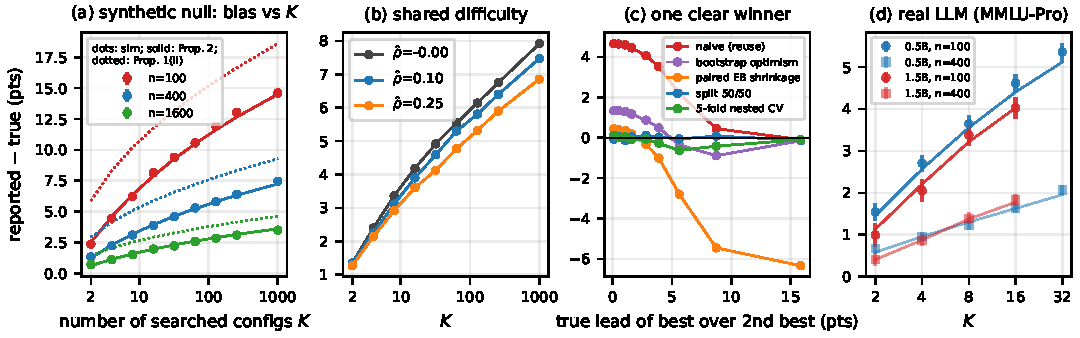
\includegraphics[width=\linewidth]{figs/fig_scaling.pdf}
\caption{Reported minus true accuracy of the selected configuration (exhaustive search; 95\% CIs). (a) Synthetic null, $\hat\rho=0.10$: simulation vs.\ Prop.~\ref{prop:null} (solid) and the Hoeffding bound (dotted). (b) Shared difficulty reduces the gap. (c) The gap vanishes when one configuration is clearly best (synthetic, $K{=}32$, $n{=}400$). (d) Real LLMs ($K=K_{\rm tot}$): dots simulation, lines Gaussian prediction from the measured covariance.}\label{fig:scaling}
\end{figure}
\begin{table}[t]
\caption{Real LLMs, tune-then-report on an $n$-question benchmark ($R{=}1000$; SH $R{=}300$). \emph{Gap} = reported $-$ true accuracy of the delivered configuration (pts, mean $\pm$ 95\% CI); \emph{Pred} = Gaussian prediction from the measured covariance (exhaustive only); \emph{Cov} = coverage (\%) of the naive Wilson 95\% interval for the delivered config's true accuracy; \emph{evals} = (config, question) evaluations used. Full grid in Table~\ref{tab:curse_full}.}\label{tab:curse}
\centering\footnotesize\setlength{\tabcolsep}{3.5pt}
\begin{tabular}{llrrrrrrr}
\toprule
Model & search & $K$ & $n$ & evals & True acc.\ (\%) & Gap (pts) & Pred & Cov \\
\midrule
0.5B & EXH & 32 & 100 & 3200 & 16.4 & +5.36 $\pm$ 0.20 & 5.12 & 73 \\
0.5B & EXH & 32 & 200 & 6400 & 16.8 & +3.50 $\pm$ 0.14 & 3.26 & 79 \\
0.5B & EXH & 32 & 400 & 12800 & 17.4 & +2.07 $\pm$ 0.10 & 1.95 & 84 \\
0.5B & EXH & 32 & 800 & 25600 & 17.7 & +1.17 $\pm$ 0.08 & 1.10 & 88 \\
0.5B & EXH & 4 & 100 & 400 & 15.9 & +2.70 $\pm$ 0.20 & 2.57 & 91 \\
0.5B & EXH & 8 & 100 & 800 & 16.3 & +3.64 $\pm$ 0.20 & 3.56 & 86 \\
0.5B & EXH & 16 & 100 & 1600 & 16.4 & +4.61 $\pm$ 0.20 & 4.40 & 78 \\
0.5B & SH & 32 & 100 & 1032 & 16.2 & +4.09 $\pm$ 0.39 & -- & 83 \\
0.5B & SH & 32 & 400 & 4000 & 17.0 & +1.57 $\pm$ 0.19 & -- & 90 \\
1.5B & EXH & 16 & 100 & 1600 & 29.6 & +4.02 $\pm$ 0.25 & 4.03 & 87 \\
1.5B & EXH & 16 & 200 & 3200 & 29.8 & +2.76 $\pm$ 0.19 & 2.69 & 87 \\
1.5B & EXH & 16 & 400 & 6400 & 29.9 & +1.83 $\pm$ 0.13 & 1.78 & 89 \\
1.5B & EXH & 16 & 800 & 12800 & 30.0 & +1.22 $\pm$ 0.09 & 1.18 & 90 \\
1.5B & EXH & 4 & 100 & 400 & 29.4 & +2.05 $\pm$ 0.27 & 2.21 & 94 \\
1.5B & EXH & 8 & 100 & 800 & 29.6 & +3.38 $\pm$ 0.25 & 3.22 & 92 \\
1.5B & SH & 16 & 100 & 808 & 29.5 & +3.61 $\pm$ 0.45 & -- & 90 \\
1.5B & SH & 16 & 400 & 3200 & 29.9 & +1.44 $\pm$ 0.25 & -- & 90 \\
\bottomrule

\end{tabular}
\end{table}
Table~\ref{tab:curse} and Fig.~\ref{fig:scaling} show a large, systematic optimism.
With $K=32$ candidates and a 100-question benchmark the reported 0.5B score exceeds the true accuracy of the delivered prompt by $5.4\pm0.2$ pts (21.8\% reported vs.\ 16.4\% true); for the 1.5B model with $K=16$ it is $4.0\pm0.3$ pts. The gap falls with $n$ roughly as $n^{-1/2}$ (0.5B, $K{=}32$: 5.4, 3.5, 2.1, 1.2 pts for $n=100,200,400,800$) and rises slowly with $K$ (0.5B, $n{=}100$: 1.6, 2.7, 3.6, 4.6, 5.4 for $K=2,4,8,16,32$). It is well predicted by the Gaussian null model with the measured covariance (e.g.\ 5.1 vs.\ 5.4 and 1.9 vs.\ 2.1 pts; over all cells with $K\ge4$ within 10\%, mean deviation 3--4\%), and the synthetic null reproduces Prop.~\ref{prop:null} to within 6.5\% (mean 1.8\%) for $K$ from 4 to 1000 and $n$ from 100 to 1600 (Fig.~\ref{fig:scaling}a, Table~\ref{tab:synth_scale}).
Three factors modulate it: (i) \emph{shared difficulty}: more correlated configurations leave less to exploit (synthetic, $K{=}32$, $n{=}100$: 10.0, 9.4, 8.5 pts at $\hat\rho=0,0.10,0.25$; real: 1.5B with $\hat\rho=0.63$ has the smaller gap at equal $K$ despite larger accuracy variance); (ii) \emph{true spread}: a clear winner removes the curse (Fig.~\ref{fig:scaling}c); (iii) \emph{search effort}: SH, which spends 2--3$\times$ fewer evaluations at $K\ge16$, has a smaller but still substantial gap (0.5B, $K{=}32$, $n{=}100$: 4.1 vs.\ 5.4 pts).
The Wilson 95\% interval of the reported score covers the delivered configuration's true accuracy only 73--88\% (0.5B, $K{=}32$) and 87--90\% (1.5B, $K{=}16$) of the time for $n\le800$.

\begin{table}[t]
\caption{Decomposition of the reported gain over an average candidate (exhaustive, $K=K_{\rm tot}$). \emph{Reported}: reported score of the delivered config minus mean true accuracy of all candidates; \emph{True}: its true accuracy minus the same; \emph{Oracle}: the best candidate's true accuracy minus the same. All in pts.}\label{tab:gain}
\centering\footnotesize
\begin{tabular}{lrrrrrr}
\toprule Model & $K$ & $n$ & Reported & True & Oracle & True/Reported (\%)\\ \midrule
0.5B & 32 & 100 & +6.53 & +1.17 & +2.93 & 18 \\
0.5B & 32 & 200 & +5.07 & +1.57 & +2.93 & 31 \\
0.5B & 32 & 400 & +4.15 & +2.08 & +2.93 & 50 \\
0.5B & 32 & 800 & +3.58 & +2.41 & +2.93 & 67 \\
1.5B & 16 & 100 & +5.55 & +1.53 & +2.36 & 28 \\
1.5B & 16 & 200 & +4.54 & +1.78 & +2.36 & 39 \\
1.5B & 16 & 400 & +3.69 & +1.86 & +2.36 & 50 \\
1.5B & 16 & 800 & +3.20 & +1.97 & +2.36 & 62 \\
\bottomrule
\end{tabular}
\end{table}
\paragraph{How much of the tuning gain is real?}
Table~\ref{tab:gain} translates the gap into the quantity practitioners report: the gain from tuning.
At $n=100$ only 18\% (0.5B) and 28\% (1.5B) of the reported gain over an average candidate is real; at $n=400$ half of it is.
In every cell the reported gain exceeds the gain of the \emph{best} candidate in the pool (Prop.~\ref{prop:bound}(i)), i.e.\ the number is unreachable by any configuration at that $n$.

\subsection{Does the gap change conclusions?}\label{sec:decisions}
\paragraph{Improvement claims.}
We declare ``tuned beats baseline'' when a one-sided paired test on the same benchmark rejects at 5\%. With the baseline equal to the \emph{best} configuration in the pool (so no candidate is truly better), the naive test makes a false claim in 12.2\% (0.5B, $K{=}31$, $n{=}200$) and 14.9\% (1.5B, $K{=}15$) of runs, against 4--5\% for $K{=}4$ (Table~\ref{tab:claims}; $n{=}800$ in Table~\ref{tab:claims_full}); the reported mean improvement is positive ($+1.9$ and $+2.1$ pts) although the true improvement is $-1.5$ and $-0.7$ pts.
With a mid-pool baseline (rank 4) the false-claim rate is 10--11\% at $K\ge15$--31, $n{=}200$ and does not shrink at $n=800$ for the 1.5B model (9.9\%).
\begin{table}[t]
\caption{Improvement claims against a fixed baseline (baseline rank = rank of its true accuracy among all configs, excluded from the search). Rep./True impr.: mean reported and true improvement of the delivered config (pts). $P_{\le0}$: \% of runs where the delivered config is truly not better. Claim / False: \% runs declaring an improvement (one-sided paired test, 5\%) and declaring it while the delivered config is truly not better. Max-$T$: simultaneous bootstrap test over the $K$ candidates.}\label{tab:claims}
\centering\footnotesize\setlength{\tabcolsep}{2.8pt}
\begin{tabular}{lrrrrrrrrrrrr}
\toprule & Base & & & Rep. & True & & \multicolumn{2}{c}{naive} & \multicolumn{2}{c}{split 50/50} & \multicolumn{2}{c}{max-$T$}\\
\cmidrule(lr){8-9}\cmidrule(lr){10-11}\cmidrule(lr){12-13}
Model & rank & $K$ & $n$ & impr. & impr. & $P_{\le0}$ & Claim & False & Claim & False & Claim & False\\ \midrule
0.5B & 1 & 4 & 200 & -0.38 & -2.19 & 100 & 2.6 & 2.6 & 2.7 & 2.7 & 0.9 & 0.9 \\
0.5B & 1 & 16 & 200 & +1.25 & -1.63 & 100 & 6.8 & 6.8 & 2.2 & 2.2 & 0.1 & 0.1 \\
0.5B & 1 & 31 & 200 & +1.95 & -1.50 & 100 & 12.2 & 12.2 & 2.6 & 2.6 & 0.3 & 0.3 \\
0.5B & 4 & 4 & 200 & +0.14 & -1.64 & 83 & 4.4 & 2.8 & 2.4 & 1.7 & 1.2 & 0.7 \\
0.5B & 4 & 16 & 200 & +1.80 & -1.07 & 72 & 11.2 & 6.9 & 3.0 & 0.9 & 1.0 & 0.5 \\
0.5B & 4 & 31 & 200 & +2.43 & -0.98 & 68 & 17.6 & 11.0 & 3.6 & 0.9 & 1.2 & 0.4 \\
1.5B & 1 & 4 & 200 & +0.42 & -0.95 & 100 & 4.4 & 4.4 & 3.4 & 3.4 & 1.0 & 1.0 \\
1.5B & 1 & 15 & 200 & +2.13 & -0.74 & 100 & 14.9 & 14.9 & 3.9 & 3.9 & 1.6 & 1.6 \\
1.5B & 4 & 4 & 200 & +0.92 & -0.53 & 76 & 7.9 & 5.5 & 4.4 & 3.0 & 3.0 & 1.6 \\
1.5B & 4 & 15 & 200 & +2.34 & -0.27 & 66 & 16.2 & 10.1 & 2.9 & 2.3 & 2.0 & 1.4 \\
\bottomrule
\end{tabular}
\end{table}
\paragraph{Comparing systems tuned with different budgets.}
Two equally good systems A and B are tuned on the same benchmark with $K_A$ and $K_B$ candidates (disjoint random subsets, so the only difference is search effort). Table~\ref{tab:systems} (App.~\ref{app:more}) shows that the harder-tuned system looks better: with $(K_A,K_B)=(16,2)$ and $n=100$ the reported gap is $+4.0$ pts (0.5B) against a true $+0.7$; A is reported ahead in 87\% of runs but is truly ahead in 63\%; at $n=400$ the reported advantage is still twice the true one ($+2.4$ vs.\ $+1.3$). With equal budgets (2 vs.\ 2) the gap is unbiased ($\approx0$), confirming that the bias is due to unequal selection pressure, not to the comparison itself. Hence a leaderboard of ``tuned-on-benchmark'' scores partly ranks tuning budgets.

\paragraph{Tuning on one subject group, deploying on another.}
Selecting on STEM questions only and deploying on non-STEM (Table~\ref{tab:shift}, App.~\ref{app:more}) adds a second, \emph{separate} gap: the delivered configuration's in-distribution true accuracy (STEM) is not its deployment accuracy.
In our matrices the two components have \emph{opposite signs} (the models are better on non-STEM subjects than on STEM), so the net reported-minus-deployed gap is small or even negative (e.g.\ 1.5B: reported 30.1\%, STEM-true 26.0\%, non-STEM 33.1\%), which would make a reported score look ``conservative'' for the wrong reason; the selection regret on the target group (best candidate there minus delivered) is 0.8--2.2 pts (0.5B) and 0.6--1.2 (1.5B).
We therefore do not claim a general direction for shift effects, only that they are not removed by any in-distribution protocol.


\subsection{Which reporting protocols are reliable?}\label{sec:protocols_results}

Table~\ref{tab:protocols} (and Fig.~\ref{fig:protocols}, App.~\ref{app:more}) compare the protocols of \S\ref{sec:protocols} on the same replicates. 
\textbf{Split reporting} is unbiased for the delivered configuration in every setting ($|{\rm bias}|\le0.35$ pts, within CIs) and has $93$--$96\%$ coverage, as Prop.~\ref{prop:split} predicts, but its intervals are wide (50/50: 14--18 pts at $n=200$).
\textbf{Nested 5-fold CV} is also unbiased (a point estimate of the \emph{procedure}, $\le0.35$ pts) with the narrowest honest interval, but Wilson intervals under-cover (82--90\%) because folds are dependent; we do not recommend its naive interval.
\textbf{Bootstrap optimism} removes roughly 70--80\% of the bias but leaves $+0.7$ to $+1.9$ pts (real/synthetic), (the .632 variant is worse, $+0.9$ to $+2.5$ pts, in the released result files); its intervals are close to nominal (95--98\%) but inherit the naive width around a centre that is still too high.
\textbf{Paired empirical-Bayes shrinkage} is the most accurate point estimate when true differences are exchangeable (synthetic: RMSE 1.8--2.5 pts vs.\ 4.6--4.8 for split 50/50) but \emph{fails when one candidate is truly better}: in the synthetic needle sweep (one candidate better by 6, 8, 12 pts; realised lead over the runner-up 3.9, 5.6, 8.7 pts) its bias becomes $-1.0$, $-2.8$, $-5.5$ pts and its coverage 96\%, 72\%, 33\% (Table~\ref{tab:needle}), and with the 1.5B matrix (one clearly worse configuration inflates the estimated spread) it over-reports by $+1.2$ pts. It cannot be used as a default.
\textbf{Max-$T$ simultaneous intervals} cover 97--99\% everywhere (also under SH) and give valid one-sided lower bounds (96--99\%) \emph{for any selection rule over the $K$ candidates}, at the price of wide intervals (17--22 pts at $n=200$; one-sided margin 10.3 vs.\ 5.7 pts for the naive bound at $K{=}32$, Table~\ref{tab:lower}; the naive lower bound covers only 70--83\% on the real matrices and 39--58\% in synthetic settings), and the corresponding improvement test is very conservative (Table~\ref{tab:claims}: 0.1--2.0\% false claims, but also only 0.4--5.8\% of the truly-better cases detected, against 2--13\% for split and 6--25\% for naive; true improvements here are $<1$ pt).
\begin{table}[t]
\caption{Protocols at $n=200$, exhaustive search over $K=32$ (synthetic) or $K=K_{\rm tot}$ (real). Bias: reported $-$ true accuracy of the config the protocol delivers (split: the config chosen on the selection half), pts $\pm$ 95\% CI; RMSE (pts); Cov: coverage of the nominal 95\% interval (\%); Width: mean interval width (pts). Split 20/80 selects on 20\% and reports on 80\%.}\label{tab:protocols}
\centering\footnotesize\setlength{\tabcolsep}{3pt}
\begin{tabular}{llrrrr}
\toprule Setting & Protocol & Bias & RMSE & Cov & Width\\ \midrule
synth null & naive (reuse) & +6.63 $\pm$ 0.16 & 6.92 & 50 & 13.5 \\
synth null & split 20/80 (sel/rep) & +0.01 $\pm$ 0.58 & 7.24 & 96 & 27.8 \\
synth null & split 50/50 & -0.17 $\pm$ 0.37 & 4.67 & 96 & 18.1 \\
synth null & 5-fold nested CV & +0.02 $\pm$ 0.36 & 4.52 & 85 & 12.9 \\
synth null & bootstrap optimism & +1.90 $\pm$ 0.20 & 3.10 & 96 & 13.6 \\
synth null & paired EB shrinkage & +0.72 $\pm$ 0.13 & 1.76 & 100 & 13.6 \\
synth null & max-$T$ simultaneous CI & -- & -- & 97 & 21.6 \\
\midrule
synth needle & naive (reuse) & +6.23 $\pm$ 0.19 & 6.65 & 55 & 13.5 \\
synth needle & split 20/80 (sel/rep) & -0.20 $\pm$ 0.59 & 7.42 & 96 & 27.9 \\
synth needle & split 50/50 & -0.32 $\pm$ 0.37 & 4.62 & 96 & 18.2 \\
synth needle & 5-fold nested CV & -0.14 $\pm$ 0.38 & 4.69 & 84 & 13.0 \\
synth needle & bootstrap optimism & +1.58 $\pm$ 0.22 & 3.17 & 96 & 13.6 \\
synth needle & paired EB shrinkage & +0.26 $\pm$ 0.17 & 2.15 & 100 & 13.6 \\
synth needle & max-$T$ simultaneous CI & -- & -- & 97 & 21.7 \\
\midrule
0.5B real & naive (reuse) & +3.50 $\pm$ 0.14 & 4.13 & 79 & 11.1 \\
0.5B real & split 20/80 (sel/rep) & +0.24 $\pm$ 0.36 & 5.74 & 96 & 22.5 \\
0.5B real & split 50/50 & +0.04 $\pm$ 0.22 & 3.53 & 96 & 14.4 \\
0.5B real & 5-fold nested CV & -0.05 $\pm$ 0.21 & 3.32 & 89 & 10.3 \\
0.5B real & bootstrap optimism & +0.74 $\pm$ 0.15 & 2.52 & 98 & 11.1 \\
0.5B real & paired EB shrinkage & +0.01 $\pm$ 0.14 & 2.21 & 99 & 11.1 \\
0.5B real & max-$T$ simultaneous CI & -- & -- & 99 & 17.2 \\
\midrule
1.5B real & naive (reuse) & +2.76 $\pm$ 0.19 & 4.10 & 87 & 12.9 \\
1.5B real & split 20/80 (sel/rep) & -0.12 $\pm$ 0.46 & 7.49 & 93 & 26.9 \\
1.5B real & split 50/50 & -0.05 $\pm$ 0.29 & 4.61 & 94 & 17.5 \\
1.5B real & 5-fold nested CV & -0.05 $\pm$ 0.23 & 3.74 & 90 & 12.5 \\
1.5B real & bootstrap optimism & +0.70 $\pm$ 0.20 & 3.26 & 95 & 13.0 \\
1.5B real & paired EB shrinkage & +1.20 $\pm$ 0.19 & 3.36 & 95 & 13.0 \\
1.5B real & max-$T$ simultaneous CI & -- & -- & 98 & 18.0 \\
\bottomrule
\end{tabular}
\end{table}

\paragraph{The price of honesty is small if the selection share is small.}
Fig.~\ref{fig:split} sweeps the fraction of the benchmark used for selection under split reporting.
Most of the error of a split report comes from the held-out part being small, not from the selection half being small: selecting on 20\% and reporting on 80\% of $n=400$ questions gives RMSE 2.1 (0.5B) / 2.6 (1.5B) pts, versus 2.6 / 2.8 for the naive full-$n$ report (bias +2.0 / +1.8), with nominal 95\% coverage, while the delivered configuration is only 1.0 (0.5B) / 0.4 (1.5B) pts less accurate than with full-$n$ selection.
Thus for $n\lesssim800$ an unbiased split report with a small selection share has \emph{lower} RMSE than the naive number; the cost shows up in interval width (about 8--10 pts at $n=400$) and in a slightly weaker delivered prompt.
\begin{figure}[t]
\centering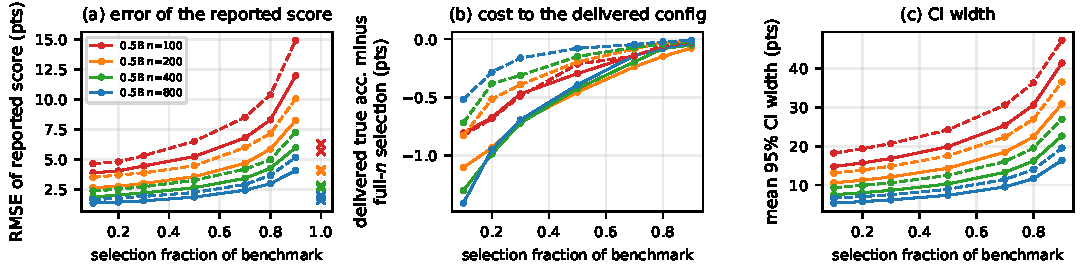
\includegraphics[width=\linewidth]{figs/fig_split.pdf}
\caption{Split reporting: sweep of the selection fraction (exhaustive search over all $K_{\rm tot}$ configs; solid 0.5B, dashed 1.5B; colours: $n=100$ red, 200 orange, 400 green, 800 blue). Crosses at 1.0 in (a): RMSE of the naive full-$n$ report.}\label{fig:split}
\end{figure}

\subsection{Validation on fresh questions}\label{sec:fresh}
The simulations treat the pool as the population. To check this against questions that were never used, we scored the same configurations on disjoint \emph{fresh} samples of MMLU-Pro (1000 questions for 0.5B, 600 for 1.5B, same length filter; 7.8 and 7.5 more CPU-hours) and (i) took the one real, un-simulated selection (best of all $K_{\rm tot}$ configurations on the full pool, i.e.\ $n=N$) and measured it on the fresh questions, and (ii) re-measured the simulated winner's curse against fresh-question accuracy instead of pool accuracy.
\begin{table}[t]
\caption{Fresh-question check. Top: the best configuration on the pool, its pool and fresh accuracy (Wilson 95\% CI), the mean over all configs of pool / fresh accuracy, its rank on the fresh questions, and the Pearson correlation / OLS slope of fresh on pool config accuracies. Bottom: gap (pts) of the naive report ($K=K_{\rm tot}$, exhaustive, $R{=}2000$) measured against pool truth (main text), raw fresh truth [95\% bootstrap CI over fresh questions and replicates], and fresh truth corrected for the level difference between the two question samples.}\label{tab:fresh}
\centering\footnotesize\setlength{\tabcolsep}{3pt}
\resizebox{\linewidth}{!}{\begin{tabular}{lrrrrlrrrrr}
\toprule Model & $K$ & $N$ & $N_f$ & Pool acc. & Fresh acc.\ [CI] & mean pool & mean fresh & Rank & $r$ & Slope\\ \midrule
0.5B & 32 & 1500 & 1000 & 18.2 & 16.6 [14.4, 19.0] & 15.3 & 14.6 & 7 & 0.74 & 0.96 \\
1.5B & 16 & 1000 & 600 & 30.4 & 26.7 [23.3, 30.3] & 28.0 & 25.0 & 3 & 0.84 & 0.59 \\
\bottomrule
\end{tabular}}\\[3pt]
\begin{tabular}{lrrrll}
\toprule Model & $K$ & $n$ & Gap, pool truth & Gap, fresh truth & Gap, fresh (level-adj.)\\ \midrule
0.5B & 32 & 100 & +5.35 & +6.17 [+4.49, +7.58] & +5.51 [+5.04, +5.90] \\
0.5B & 32 & 200 & +3.43 & +4.34 [+2.90, +5.80] & +3.68 [+3.02, +4.28] \\
0.5B & 32 & 400 & +2.03 & +3.05 [+1.26, +4.73] & +2.38 [+1.54, +3.13] \\
0.5B & 32 & 800 & +1.19 & +2.30 [+0.56, +4.24] & +1.63 [+0.66, +2.69] \\
1.5B & 16 & 100 & +4.06 & +7.83 [+4.75, +10.76] & +4.79 [+4.24, +5.30] \\
1.5B & 16 & 200 & +2.82 & +6.67 [+3.69, +9.10] & +3.64 [+3.04, +4.25] \\
1.5B & 16 & 400 & +1.77 & +5.64 [+2.84, +8.27] & +2.60 [+1.96, +3.25] \\
1.5B & 16 & 800 & +1.26 & +5.16 [+2.64, +8.29] & +2.12 [+1.39, +2.93] \\
\bottomrule
\end{tabular}
\end{table}
The single real selection regresses as predicted but is weak evidence by itself (one draw): the pool-best configuration scores 18.2\% on the pool and 16.6\% on fresh questions for 0.5B (CI 14.4--19.0, rank 7 of 32), and 30.4\% vs.\ 26.7\% (CI 23.3--30.3, rank 3 of 16) for 1.5B; its lead over the average configuration shrinks from $+2.9$ to $+2.0$ and from $+2.4$ to $+1.7$ pts. Configuration accuracies on the two question sets correlate ($r=0.74$, $0.84$) with attenuation (slope 0.96, 0.59), as expected from regression to the mean.
The simulated gap against fresh truth is positive and as large as or larger than against pool truth (Table~\ref{tab:fresh}, bottom). The fresh samples are also easier or harder overall than the pool (config-mean lower by 0.7 pts for 0.5B, 3.0 pts for 1.5B; question-sampling variation), a common offset that we remove in the last column: gaps of 5.5 vs.\ 5.4 ($n{=}100$) and 2.4 vs.\ 2.0 ($n{=}400$) pts for 0.5B, and 4.8 vs.\ 4.1 and 2.6 vs.\ 1.8 for 1.5B.
Pool truth treats the pool's own sampling luck as real quality (understating the gap); benchmarks drawn from the pool inherit that luck while fresh truth does not (overstating it); we read the two as a bracket, up to about 0.8 pts wide at $n{=}400$. The conclusion---a gap of several points at $n\le200$ and 2--3 points at $n{=}400$---is not an artefact of the finite pool, and the pool-truth numbers of Sec.~\ref{sec:magnitude} are the lower end.


\section{Discussion and limitations}\label{sec:limits}
\paragraph{Practical reading.}
A benchmark score that was also used to choose among $K$ candidates is an upper estimate whose optimism is of order $\sigma\sqrt{(1-\rho)/n}\sqrt{2\ln K}$: several points for $n\le200$ even with 16--32 candidates. Recommendations, each tested above: (1) report $K$ and $n$ with the score; (2) when questions are scarce, hold out a share (20--50\%) of the benchmark \emph{after} fixing the search and report its score and interval, valid for any optimiser including a human in the loop; (3) use max-$T$/Bonferroni bounds if a guarantee over the candidate set is needed, accepting conservativeness; (4) do not compare systems with different tuning budgets on the tuning benchmark; (5) do not trust bootstrap-optimism or empirical-Bayes corrections unless no candidate is clearly better.

\paragraph{Limitations.}
\emph{Models and tasks.} Two small models (the 0.5B is near chance) and one benchmark (MMLU-Pro, short questions) with letter-logit scoring rather than generation or chain-of-thought; larger models have different $\rho$ and spread, so the quantitative gaps (4--5 pts) should not be transferred. The formulas need only $\sigma$, $\hat\rho$, $n$, $K$, measurable from cached outcomes.
\emph{Search space and optimisers.} Candidates are random draws from a small grid of five knobs (true sd between candidates 1.5--2.7 pts), searched exhaustively or by successive halving. DSPy/MIPRO-style optimisers, whose proposals are adaptive and potentially far more numerous, were not run; Prop.~\ref{prop:bound} and split reporting apply to them unchanged, the numbers in Table~\ref{tab:curse} do not, and their effective $K$ is unknown, itself an argument for split reporting.
\emph{Simulation design.} The pool (1000/1500 questions) is the population and benchmarks are drawn with replacement; \S\ref{sec:fresh} and App.~\ref{app:oos} check this against disjoint questions and the without-replacement analogue, which bracket the pool estimate; the decision experiments use pool truth only. Replicate counts give s.e.\ of 0.05--0.1 pt for gaps; coverages are accurate to about $\pm1.5$ pts. Tests use the normal approximation for paired differences.
\emph{Protocols.} Max-$T$ and the Gaussian prediction assume a fixed candidate set and large $n$; the Gaussian prediction uses the population covariance and validates the mechanism, not a practical estimator. The shift experiment uses one split whose direction is specific to our models. We did not study repeated adaptive use of one hold-out, multiple benchmarks, or non-binary metrics. Pool size and $K_{\rm tot}$ differ between the models (1500/1000, 32/16) purely for CPU budget; no GPU or API was used.

\paragraph{Conclusion.}
Reporting the tuned score on the tuning questions is optimistic in a quantitatively predictable way, large relative to the differences practitioners care about, and able to reverse comparisons; a split report with a small selection share is a cheap, search-agnostic remedy with exact validity and a measurable price, whereas bootstrap-optimism and shrinkage corrections are not dependable.


\label{endmain}
\bibliographystyle{plainnat}
\bibliography{refs}

\appendix
\section{Additional results}\label{app:more}
\begin{table}[h]
\caption{Full version of Table~\ref{tab:curse} (all searched $K$ and $n$; SH rows have $R{=}300$).}\label{tab:curse_full}
\centering\footnotesize\setlength{\tabcolsep}{3.5pt}
\begin{tabular}{llrrrrrrrr}
\toprule Model & search & $K$ & $n$ & evals & True acc.\ (\%) & Reported (\%) & Gap (pts) & Pred & Cov \\ \midrule
0.5B & EXH & 4 & 100 & 400 & 15.9 & 18.6 & +2.70 $\pm$ 0.20 & 2.57 & 91 \\
0.5B & EXH & 16 & 100 & 1600 & 16.4 & 21.0 & +4.61 $\pm$ 0.20 & 4.40 & 78 \\
0.5B & EXH & 32 & 100 & 3200 & 16.4 & 21.8 & +5.36 $\pm$ 0.20 & 5.12 & 73 \\
0.5B & EXH & 4 & 200 & 800 & 16.2 & 17.8 & +1.58 $\pm$ 0.15 & 1.63 & 93 \\
0.5B & EXH & 16 & 200 & 3200 & 16.8 & 19.7 & +2.95 $\pm$ 0.14 & 2.79 & 83 \\
0.5B & EXH & 32 & 200 & 6400 & 16.8 & 20.3 & +3.50 $\pm$ 0.14 & 3.26 & 79 \\
0.5B & EXH & 4 & 400 & 1600 & 16.4 & 17.4 & +0.96 $\pm$ 0.11 & 0.96 & 94 \\
0.5B & EXH & 16 & 400 & 6400 & 17.1 & 18.8 & +1.63 $\pm$ 0.11 & 1.63 & 87 \\
0.5B & EXH & 32 & 400 & 12800 & 17.4 & 19.4 & +2.07 $\pm$ 0.10 & 1.95 & 84 \\
0.5B & EXH & 4 & 800 & 3200 & 16.6 & 17.1 & +0.47 $\pm$ 0.08 & 0.52 & 94 \\
0.5B & EXH & 16 & 800 & 12800 & 17.5 & 18.5 & +0.96 $\pm$ 0.08 & 0.87 & 90 \\
0.5B & EXH & 32 & 800 & 25600 & 17.7 & 18.9 & +1.17 $\pm$ 0.08 & 1.10 & 88 \\
0.5B & SH & 4 & 100 & 400 & 15.8 & 18.3 & +2.49 $\pm$ 0.37 & -- & 91 \\
0.5B & SH & 16 & 100 & 808 & 16.1 & 19.8 & +3.70 $\pm$ 0.39 & -- & 84 \\
0.5B & SH & 32 & 100 & 1032 & 16.2 & 20.3 & +4.09 $\pm$ 0.39 & -- & 83 \\
0.5B & SH & 4 & 200 & 800 & 16.1 & 17.7 & +1.59 $\pm$ 0.27 & -- & 93 \\
0.5B & SH & 16 & 200 & 1600 & 16.6 & 18.8 & +2.19 $\pm$ 0.28 & -- & 90 \\
0.5B & SH & 32 & 200 & 2016 & 16.5 & 19.3 & +2.81 $\pm$ 0.29 & -- & 81 \\
0.5B & SH & 4 & 400 & 1600 & 16.4 & 17.4 & +0.93 $\pm$ 0.20 & -- & 93 \\
0.5B & SH & 16 & 400 & 3200 & 17.1 & 18.4 & +1.33 $\pm$ 0.18 & -- & 93 \\
0.5B & SH & 32 & 400 & 4000 & 17.0 & 18.6 & +1.57 $\pm$ 0.19 & -- & 90 \\
0.5B & SH & 4 & 800 & 3200 & 16.5 & 16.9 & +0.40 $\pm$ 0.14 & -- & 95 \\
0.5B & SH & 16 & 800 & 6400 & 17.2 & 18.0 & +0.77 $\pm$ 0.14 & -- & 92 \\
0.5B & SH & 32 & 800 & 8000 & 17.3 & 18.4 & +1.08 $\pm$ 0.14 & -- & 89 \\
1.5B & EXH & 4 & 100 & 400 & 29.4 & 31.5 & +2.05 $\pm$ 0.27 & 2.21 & 94 \\
1.5B & EXH & 16 & 100 & 1600 & 29.6 & 33.6 & +4.02 $\pm$ 0.25 & 4.03 & 87 \\
1.5B & EXH & 4 & 200 & 800 & 29.5 & 30.9 & +1.35 $\pm$ 0.20 & 1.41 & 93 \\
1.5B & EXH & 16 & 200 & 3200 & 29.8 & 32.6 & +2.76 $\pm$ 0.19 & 2.69 & 87 \\
1.5B & EXH & 4 & 400 & 1600 & 29.7 & 30.6 & +0.87 $\pm$ 0.13 & 0.88 & 94 \\
1.5B & EXH & 16 & 400 & 6400 & 29.9 & 31.7 & +1.83 $\pm$ 0.13 & 1.78 & 89 \\
1.5B & EXH & 4 & 800 & 3200 & 29.8 & 30.4 & +0.53 $\pm$ 0.10 & 0.54 & 95 \\
1.5B & EXH & 16 & 800 & 12800 & 30.0 & 31.2 & +1.22 $\pm$ 0.09 & 1.18 & 90 \\
1.5B & SH & 4 & 100 & 400 & 29.3 & 31.3 & +1.96 $\pm$ 0.50 & -- & 93 \\
1.5B & SH & 16 & 100 & 808 & 29.5 & 33.1 & +3.61 $\pm$ 0.45 & -- & 90 \\
1.5B & SH & 4 & 200 & 800 & 29.7 & 31.2 & +1.52 $\pm$ 0.34 & -- & 94 \\
1.5B & SH & 16 & 200 & 1600 & 29.7 & 32.1 & +2.37 $\pm$ 0.33 & -- & 91 \\
1.5B & SH & 4 & 400 & 1600 & 29.6 & 30.3 & +0.68 $\pm$ 0.25 & -- & 96 \\
1.5B & SH & 16 & 400 & 3200 & 29.9 & 31.3 & +1.44 $\pm$ 0.25 & -- & 90 \\
1.5B & SH & 4 & 800 & 3200 & 29.8 & 30.4 & +0.56 $\pm$ 0.17 & -- & 95 \\
1.5B & SH & 16 & 800 & 6400 & 30.0 & 31.0 & +0.95 $\pm$ 0.17 & -- & 91 \\
\bottomrule
\end{tabular}
\end{table}

\subsection{Synthetic experiments}\label{app:synth}
\paragraph{Generator.} $Y_{ci}\sim\mathrm{Bernoulli}(\sigma(\mathrm{logit}(0.25)+a_i+b_c+g_{ci}))$ with shared difficulty $a_i\sim\mathcal N(0,s_a^2)$, interaction $g_{ci}\sim\mathcal N(0,s_g^2)$, $s_a^2+s_g^2=4$, configuration effects $b_c$ (zero for the null; $\mathcal N(0,\tau^2)$ for ``spread''; one configuration raised by $\delta$ for ``needle''; Laplace(scale 1 pt) for ``heavy''), population of $4\times10^4$ questions, benchmarks drawn from it with replacement.
$\hat\rho$ is the measured mean pairwise covariance divided by the mean variance.
\begin{table}[h]
\caption{Synthetic null: bias of the naive report in pts (null prediction of Prop.~\ref{prop:null} in parentheses) [coverage of the naive 95\% Wilson interval, \%], by number of candidates $K$ and benchmark size $n$.}\label{tab:synth_scale}
\centering\footnotesize
\begin{tabular}{rrlll}
\toprule $\hat\rho$ & $K$ & $n=100$ & $n=400$ & $n=1600$\\ \midrule
0.00 & 4 & 4.58 (4.87) [93] & 2.40 (2.44) [91] & 1.14 (1.22) [91] \\
0.00 & 32 & 10.01 (9.79) [44] & 4.92 (4.90) [44] & 2.39 (2.45) [47] \\
0.00 & 256 & 13.84 (13.38) [0] & 6.75 (6.69) [1] & 3.31 (3.34) [1] \\
0.00 & 1000 & 15.59 (15.34) [0] & 7.91 (7.67) [0] & 3.81 (3.83) [0] \\
0.11 & 4 & 4.48 (4.60) [92] & 2.25 (2.30) [90] & 1.13 (1.15) [90] \\
0.10 & 32 & 9.40 (9.27) [51] & 4.59 (4.64) [52] & 2.23 (2.32) [55] \\
0.11 & 256 & 13.04 (12.67) [4] & 6.40 (6.33) [6] & 3.11 (3.17) [10] \\
0.11 & 1000 & 14.60 (14.50) [1] & 7.47 (7.25) [0] & 3.51 (3.62) [2] \\
0.26 & 4 & 4.36 (4.20) [91] & 2.14 (2.10) [90] & 1.07 (1.05) [91] \\
0.25 & 32 & 8.51 (8.47) [62] & 4.13 (4.24) [63] & 2.03 (2.12) [62] \\
0.26 & 256 & 11.92 (11.56) [19] & 5.90 (5.78) [20] & 2.82 (2.89) [26] \\
0.26 & 1000 & 13.08 (13.21) [11] & 6.86 (6.61) [5] & 3.22 (3.30) [8] \\
\bottomrule
\end{tabular}
\end{table}
\begin{table}[h]
\caption{``Needle'' sweep: one of $K=32$ synthetic candidates is better by $\delta$ pts, $n=400$. Lead: realised true lead over the runner-up. Bias (pts) of each protocol; EB also shows coverage (\%) of its nominal 95\% interval.}\label{tab:needle}
\centering\footnotesize
\begin{tabular}{rrrrrrr}
\toprule $\delta$ & Lead & naive & bootstrap opt. & EB (cov) & nested CV & split 50/50\\ \midrule
0 & 0.1 & +4.65 & +1.33 & +0.44 (100) & +0.12 & -0.07 \\
1 & 0.5 & +4.64 & +1.33 & +0.39 (100) & +0.02 & +0.05 \\
2 & 1.1 & +4.60 & +1.29 & +0.36 (100) & +0.04 & -0.13 \\
3 & 1.6 & +4.45 & +1.17 & +0.18 (100) & -0.09 & +0.04 \\
4 & 2.8 & +4.06 & +0.87 & -0.32 (100) & -0.07 & +0.11 \\
6 & 3.9 & +3.52 & +0.49 & -1.01 (96) & -0.27 & +0.03 \\
8 & 5.6 & +2.19 & -0.36 & -2.79 (72) & -0.63 & -0.06 \\
12 & 8.7 & +0.45 & -0.89 & -5.45 (33) & -0.41 & +0.08 \\
20 & 15.9 & -0.09 & -0.15 & -6.34 (28) & -0.10 & -0.12 \\
\bottomrule
\end{tabular}
\end{table}
\begin{table}[h]
\caption{One-sided 95\% lower bounds for the delivered config's true accuracy: coverage \% (mean margin $\hat\mu_{\hat c}-\mathrm{bound}$ in pts). Naive: $\hat\mu-1.645\,\widehat{\rm se}$; max-$T$: bootstrap quantile of $\max_c T_c$; Hoeffding--Bonferroni: $\sqrt{\ln(K/0.05)/(2n)}$. Top: synthetic, bottom: real (exhaustive).}\label{tab:lower}
\centering\footnotesize
\begin{tabular}{llrrrrr}
\toprule Regime & search & $K$ & $n$ & naive & max-$T$ & Hoeffding--Bonf.\\ \midrule
null & EXH & 32 & 200 & 32 (5.7) & 96 (10.3) & 100 (12.7) \\
null & EXH & 32 & 800 & 32 (2.8) & 97 (5.0) & 100 (6.4) \\
null & EXH & 256 & 400 & 2 (4.0) & 97 (8.7) & 99 (10.3) \\
null & SH & 32 & 200 & 63 (5.7) & 98 (10.2) & 100 (12.7) \\
spread (sd 3 pts) & EXH & 32 & 200 & 58 (5.8) & 97 (10.4) & 100 (12.7) \\
spread (sd 3 pts) & EXH & 32 & 800 & 72 (2.8) & 98 (5.1) & 100 (6.4) \\
spread (sd 3 pts) & EXH & 256 & 400 & 42 (4.1) & 99 (8.8) & 100 (10.3) \\
needle (+5 pts) & EXH & 32 & 200 & 39 (5.7) & 96 (10.3) & 100 (12.7) \\
needle (+5 pts) & EXH & 32 & 800 & 62 (2.8) & 98 (5.1) & 100 (6.4) \\
needle (+5 pts) & EXH & 256 & 400 & 12 (4.0) & 97 (8.7) & 99 (10.3) \\
heavy-tailed & EXH & 32 & 200 & 44 (5.7) & 97 (10.3) & 100 (12.7) \\
heavy-tailed & EXH & 32 & 800 & 48 (2.8) & 97 (5.0) & 100 (6.4) \\
heavy-tailed & EXH & 256 & 400 & 24 (4.0) & 98 (8.8) & 99 (10.3) \\
\bottomrule
\end{tabular}\\[2pt]
\begin{tabular}{lrrrrr}
\toprule Model & $K$ & $n$ & naive & max-$T$ & Hoeffding--Bonf.\\ \midrule
0.5B & 32 & 100 & 70 (6.8) & 98 (12.2) & 100 (18.0) \\
0.5B & 32 & 200 & 71 (4.7) & 99 (8.3) & 100 (12.7) \\
0.5B & 32 & 400 & 77 (3.2) & 99 (5.7) & 100 (9.0) \\
1.5B & 16 & 100 & 83 (7.7) & 97 (11.8) & 100 (17.0) \\
1.5B & 16 & 200 & 82 (5.4) & 97 (8.3) & 100 (12.0) \\
1.5B & 16 & 400 & 83 (3.8) & 96 (5.8) & 100 (8.5) \\
\bottomrule
\end{tabular}
\end{table}

\begin{figure}[h]
\centering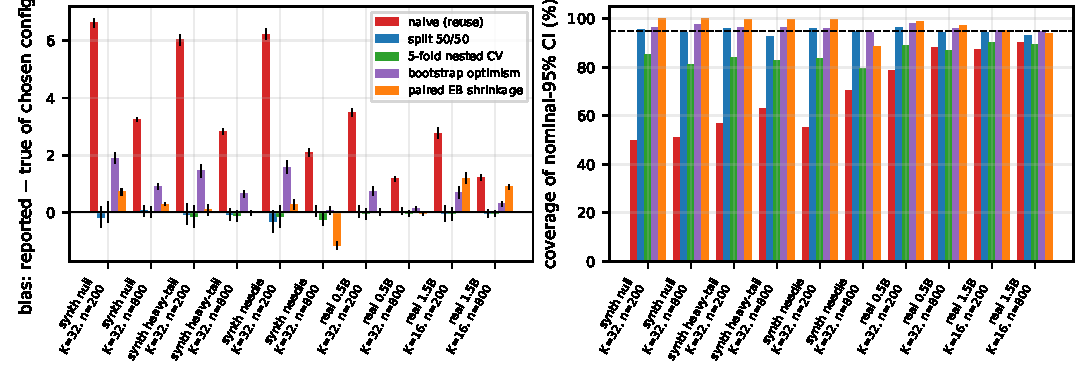
\includegraphics[width=\linewidth]{figs/fig_protocols.pdf}
\caption{Bias (left) and nominal-95\% interval coverage (right) of protocols across synthetic regimes and real LLMs (exhaustive search, $K=32$ or $K_{\rm tot}=16$). Error bars: 95\% CI over replicates. Dashed line: 95\%.}\label{fig:protocols}
\end{figure}
\begin{table}[h]
\caption{Select on STEM questions ($n$ per benchmark), deliver, evaluate on STEM and non-STEM (exhaustive). Gap = reported $-$ STEM-true, Shift = STEM-true $-$ non-STEM-true (pts, mean $\pm$ 95\% CI); Regret = best candidate's non-STEM accuracy $-$ delivered config's (pts).}\label{tab:shift}
\centering\footnotesize
\begin{tabular}{lrrrrrrrr}
\toprule Model & $K$ & $n$ & Reported & STEM & non-STEM & Gap & Shift & Regret\\ \midrule
0.5B & 4 & 100 & 17.2 & 14.5 & 17.4 & +2.71 $\pm$ 0.19 & -2.96 $\pm$ 0.07 & 1.04 \\
0.5B & 4 & 400 & 15.9 & 14.9 & 17.7 & +0.99 $\pm$ 0.10 & -2.74 $\pm$ 0.07 & 0.81 \\
0.5B & 16 & 100 & 19.4 & 14.9 & 17.7 & +4.54 $\pm$ 0.18 & -2.81 $\pm$ 0.07 & 1.92 \\
0.5B & 16 & 400 & 17.5 & 15.7 & 18.3 & +1.80 $\pm$ 0.10 & -2.58 $\pm$ 0.07 & 1.37 \\
0.5B & 32 & 100 & 20.3 & 15.0 & 17.7 & +5.28 $\pm$ 0.18 & -2.70 $\pm$ 0.07 & 2.19 \\
0.5B & 32 & 400 & 18.0 & 15.8 & 18.4 & +2.15 $\pm$ 0.10 & -2.56 $\pm$ 0.06 & 1.56 \\
1.5B & 4 & 100 & 27.7 & 25.6 & 33.1 & +2.14 $\pm$ 0.26 & -7.52 $\pm$ 0.09 & 0.67 \\
1.5B & 4 & 400 & 26.7 & 26.0 & 33.2 & +0.72 $\pm$ 0.13 & -7.18 $\pm$ 0.07 & 0.61 \\
1.5B & 16 & 100 & 30.1 & 26.0 & 33.1 & +4.15 $\pm$ 0.24 & -7.19 $\pm$ 0.08 & 1.21 \\
1.5B & 16 & 400 & 28.1 & 26.3 & 33.2 & +1.75 $\pm$ 0.12 & -6.88 $\pm$ 0.06 & 1.15 \\
\bottomrule
\end{tabular}
\end{table}
\begin{table}[h]
\caption{Full version of Table~\ref{tab:claims} (all $K$ and $n$).}\label{tab:claims_full}
\centering\footnotesize\setlength{\tabcolsep}{2.8pt}
\begin{tabular}{lrrrrrrrrrrrr}
\toprule & Base & & & Rep. & True & & \multicolumn{2}{c}{naive} & \multicolumn{2}{c}{split 50/50} & \multicolumn{2}{c}{max-$T$}\\
\cmidrule(lr){8-9}\cmidrule(lr){10-11}\cmidrule(lr){12-13}
Model & rank & $K$ & $n$ & impr. & impr. & $P_{\le0}$ & Claim & False & Claim & False & Claim & False\\ \midrule
0.5B & 1 & 4 & 200 & -0.38 & -2.19 & 100 & 2.6 & 2.6 & 2.7 & 2.7 & 0.9 & 0.9 \\
0.5B & 1 & 4 & 800 & -1.22 & -1.75 & 100 & 1.1 & 1.1 & 0.9 & 0.9 & 0.4 & 0.4 \\
0.5B & 1 & 16 & 200 & +1.25 & -1.63 & 100 & 6.8 & 6.8 & 2.2 & 2.2 & 0.1 & 0.1 \\
0.5B & 1 & 16 & 800 & +0.15 & -0.93 & 100 & 5.2 & 5.2 & 1.7 & 1.7 & 0.3 & 0.3 \\
0.5B & 1 & 31 & 200 & +1.95 & -1.50 & 100 & 12.2 & 12.2 & 2.6 & 2.6 & 0.3 & 0.3 \\
0.5B & 1 & 31 & 800 & +0.46 & -0.70 & 100 & 6.6 & 6.6 & 1.9 & 1.9 & 0.4 & 0.4 \\
0.5B & 4 & 4 & 200 & +0.14 & -1.64 & 83 & 4.4 & 2.8 & 2.4 & 1.7 & 1.2 & 0.7 \\
0.5B & 4 & 4 & 800 & -0.76 & -1.30 & 77 & 4.2 & 1.3 & 3.5 & 1.2 & 1.3 & 0.3 \\
0.5B & 4 & 16 & 200 & +1.80 & -1.07 & 72 & 11.2 & 6.9 & 3.0 & 0.9 & 1.0 & 0.5 \\
0.5B & 4 & 16 & 800 & +0.60 & -0.39 & 54 & 12.5 & 4.2 & 4.5 & 1.1 & 1.3 & 0.2 \\
0.5B & 4 & 31 & 200 & +2.43 & -0.98 & 68 & 17.6 & 11.0 & 3.6 & 0.9 & 1.2 & 0.4 \\
0.5B & 4 & 31 & 800 & +0.94 & -0.13 & 43 & 16.2 & 4.7 & 4.7 & 1.5 & 1.2 & 0.3 \\
1.5B & 1 & 4 & 200 & +0.42 & -0.95 & 100 & 4.4 & 4.4 & 3.4 & 3.4 & 1.0 & 1.0 \\
1.5B & 1 & 4 & 800 & -0.12 & -0.70 & 100 & 4.5 & 4.5 & 3.4 & 3.4 & 1.5 & 1.5 \\
1.5B & 1 & 15 & 200 & +2.13 & -0.74 & 100 & 14.9 & 14.9 & 3.9 & 3.9 & 1.6 & 1.6 \\
1.5B & 1 & 15 & 800 & +0.74 & -0.49 & 100 & 11.0 & 11.0 & 3.2 & 3.2 & 0.8 & 0.8 \\
1.5B & 4 & 4 & 200 & +0.92 & -0.53 & 76 & 7.9 & 5.5 & 4.4 & 3.0 & 3.0 & 1.6 \\
1.5B & 4 & 4 & 800 & +0.26 & -0.22 & 69 & 6.3 & 3.5 & 4.2 & 2.5 & 2.0 & 1.1 \\
1.5B & 4 & 15 & 200 & +2.34 & -0.27 & 66 & 16.2 & 10.1 & 2.9 & 2.3 & 2.0 & 1.4 \\
1.5B & 4 & 15 & 800 & +1.11 & +0.00 & 56 & 17.7 & 9.9 & 5.9 & 2.8 & 2.9 & 1.2 \\
\bottomrule
\end{tabular}
\end{table}

\begin{table}[h]
\caption{Two systems tuned on the same $n$-question benchmark with $K_A$ vs.\ $K_B$ random candidates. Rep./True gap: mean reported and true accuracy difference A$-$B (pts). $P_{\rm rep}$, $P_{\rm true}$: \% runs with reported / true gap $>0$. Claim: \% runs where a one-sided paired test (5\%) says A $>$ B; False: same, restricted to runs where A is truly not better. Naive = same benchmark for selection and test; split = select on half, test on other half.}\label{tab:systems}
\centering\footnotesize\setlength{\tabcolsep}{3pt}
\begin{tabular}{lrrrrrrrrrrr}
\toprule & & & & Rep. & True & & & \multicolumn{2}{c}{naive} & \multicolumn{2}{c}{split}\\
\cmidrule(lr){9-10}\cmidrule(lr){11-12}
Model & $K_A$ & $K_B$ & $n$ & gap & gap & $P_{\rm rep}$ & $P_{\rm true}$ & Claim & False & Claim & False\\ \midrule
0.5B & 16 & 2 & 100 & +4.00 & +0.74 & 87 & 63 & 16.8 & 11.7 & 8.0 & 3.8 \\
0.5B & 16 & 2 & 400 & +2.38 & +1.27 & 87 & 76 & 30.4 & 7.6 & 15.9 & 3.0 \\
0.5B & 16 & 2 & 800 & +2.20 & +1.62 & 88 & 81 & 46.9 & 3.7 & 21.4 & 1.3 \\
0.5B & 8 & 2 & 100 & +2.62 & +0.59 & 73 & 62 & 9.9 & 3.7 & 7.7 & 3.8 \\
0.5B & 8 & 2 & 400 & +1.81 & +1.04 & 77 & 69 & 23.4 & 3.6 & 13.2 & 1.8 \\
0.5B & 8 & 2 & 800 & +1.53 & +1.10 & 78 & 71 & 34.4 & 4.8 & 20.7 & 0.9 \\
0.5B & 2 & 2 & 100 & -0.03 & -0.02 & 46 & 47 & 3.8 & 1.3 & 6.8 & 2.0 \\
0.5B & 2 & 2 & 400 & +0.11 & +0.13 & 50 & 52 & 9.9 & 1.0 & 9.4 & 1.7 \\
0.5B & 2 & 2 & 800 & +0.06 & +0.05 & 50 & 51 & 15.6 & 1.0 & 14.3 & 2.0 \\
1.5B & 8 & 2 & 100 & +2.79 & +0.54 & 77 & 57 & 14.5 & 7.9 & 9.6 & 5.1 \\
1.5B & 8 & 2 & 400 & +1.57 & +0.65 & 78 & 63 & 20.9 & 7.9 & 11.2 & 4.1 \\
1.5B & 8 & 2 & 800 & +1.29 & +0.63 & 78 & 64 & 26.4 & 5.2 & 14.3 & 2.6 \\
1.5B & 2 & 2 & 100 & +0.02 & +0.04 & 45 & 49 & 5.3 & 2.7 & 8.2 & 4.3 \\
1.5B & 2 & 2 & 400 & +0.02 & +0.00 & 47 & 47 & 10.7 & 2.1 & 8.6 & 2.1 \\
1.5B & 2 & 2 & 800 & -0.03 & -0.01 & 48 & 48 & 15.6 & 1.9 & 11.7 & 2.5 \\
\bottomrule
\end{tabular}
\end{table}

\begin{table}[h]
\caption{Protocols in the synthetic ``spread'' regime (configuration effects $\mathcal N(0,3\text{ pts}^2)$, $K{=}32$, $n{=}200$); columns as in Table~\ref{tab:protocols}.}\label{tab:protocols_spread}
\centering\footnotesize
\begin{tabular}{llrrrr}
\toprule Setting & Protocol & Bias & RMSE & Cov & Width\\ \midrule
synth spread & naive (reuse) & +5.30 $\pm$ 0.20 & 5.84 & 74 & 13.6 \\
synth spread & split 20/80 (sel/rep) & -0.14 $\pm$ 0.64 & 7.93 & 94 & 28.4 \\
synth spread & split 50/50 & +0.04 $\pm$ 0.38 & 4.75 & 95 & 18.5 \\
synth spread & 5-fold nested CV & -0.35 $\pm$ 0.39 & 4.87 & 82 & 13.2 \\
synth spread & bootstrap optimism & +1.10 $\pm$ 0.24 & 3.15 & 96 & 13.7 \\
synth spread & paired EB shrinkage & +0.18 $\pm$ 0.20 & 2.49 & 99 & 13.7 \\
synth spread & max-$T$ simultaneous CI & -- & -- & 98 & 21.8 \\
\bottomrule
\end{tabular}
\end{table}

\subsection{Pool truth vs.\ out-of-sample truth}\label{app:oos}
The pool is finite, so the benchmark sample $S$ overlaps the pool-mean truth. Re-measuring the same replicates against the accuracy of the delivered configuration on the pool questions \emph{not} in $S$ (without-replacement analogue; it is anti-correlated with the in-sample accuracy by construction and hence biased upwards in gap) gives the following; the pool-truth gap of the main text is the exact i.i.d.\ quantity, this table is the upper end of the bracket.
\begin{table}[h]
\caption{Gap (pts) of naive and bootstrap-corrected reports against pool truth and against out-of-sample truth ($K=K_{\rm tot}$, exhaustive).}\label{tab:oos}
\centering\footnotesize
\begin{tabular}{lrrrrr}
\toprule Model & $n$ & naive (pool) & naive (oos) & boot.\ opt.\ (pool) & boot.\ opt.\ (oos)\\ \midrule
0.5B & 100 & +5.36 & +5.71 & +1.19 & +1.54 \\
0.5B & 400 & +2.07 & +2.60 & +0.33 & +0.87 \\
0.5B & 800 & +1.17 & +1.81 & +0.14 & +0.78 \\
1.5B & 100 & +4.02 & +4.43 & +0.99 & +1.40 \\
1.5B & 400 & +1.83 & +2.59 & +0.44 & +1.19 \\
1.5B & 800 & +1.22 & +2.23 & +0.30 & +1.31 \\
\bottomrule
\end{tabular}
\end{table}

\section{Reproducibility}\label{app:repro}
\paragraph{Environment.} Python 3.11, torch 2.15.0+cpu, transformers 5.22.2, numpy 2.4.6, scipy 1.17.1, pandas 3.0.6, pyarrow 26.0.1, matplotlib 3.11.2; Intel Xeon Gold 6230 (40 logical cores shared with other jobs, 251 GB RAM), no GPU. Data: \texttt{TIGER-Lab/MMLU-Pro} revision \texttt{b189ec765aa7ed75c8acfea42df31fdae71f97be} (MIT licence); models \texttt{Qwen/Qwen2.5-\{0.5,1.5\}B-Instruct} (Apache-2.0 for 0.5B and 1.5B), fp32. Seeds: pool/config seed 0; simulation seeds are in the scripts (\texttt{--seed}).
\paragraph{Compute actually used.} LLM scoring (4 threads per job, CPU contention from other tenants; wall-clock): 7.3 h (0.5B, $32\times1500$), 5.8 h (1.5B, $16\times1000$), plus the fresh-question matrices (\S\ref{sec:fresh}; run concurrently: 7.8 h for $32\times1000$ and 7.5 h for $16\times600$), i.e.\ 28.4 job wall-hours in total (\texttt{results/compute\_usage.txt}); statistical simulations: about 0.3 CPU-hours per real-data experiment and a few CPU-hours for the synthetic study. Preliminary runs not in the paper: speed/accuracy checks on 96 questions (including torch int8 dynamic quantisation, which we abandoned because it halved accuracy), and a first synthetic run (superseded after adding the needle-size sweep and $\mu$-spread diagnostics; no results were dropped). No hyperparameter of any protocol was tuned on the reported results.
\paragraph{Scripts $\to$ outputs.} See \texttt{README.md} in the code package for commands and expected runtimes.
\begin{center}\footnotesize\begin{tabular}{ll}
\toprule Output & Script\\ \midrule
correctness matrices & \texttt{code/get\_data.py}, \texttt{code/run\_scoring.sh}, \texttt{code/run\_fresh*.sh} ($\to$ \texttt{score.py}, \texttt{prompts.py})\\
Fig.~\ref{fig:scaling}, Tab.~\ref{tab:curse},\ref{tab:gain},\ref{tab:curse_full} & \texttt{exp\_real.py}, \texttt{exp\_synth.py}, \texttt{make\_report.py}\\
Tab.~\ref{tab:claims}--\ref{tab:shift} & \texttt{exp\_decisions.py}, \texttt{make\_report.py}\\
Tab.~\ref{tab:protocols}, Fig.~\ref{fig:protocols}, Tab.~\ref{tab:synth_scale}--\ref{tab:lower} & \texttt{exp\_real.py}, \texttt{exp\_synth.py}, \texttt{make\_report.py}\\
Fig.~\ref{fig:split} & \texttt{exp\_split.py}, \texttt{make\_report.py}\\
Sec.~\ref{sec:fresh} & \texttt{exp\_fresh.py}, \texttt{make\_report.py}\\
Tab.~\ref{tab:oos} & \texttt{exp\_real.py} (oos fields), \texttt{make\_report.py}\\
matrix statistics (\S\ref{sec:setup}) & \texttt{describe\_matrix.py}\\
\bottomrule\end{tabular}\end{center}
\paragraph{Literature handling.} Only the starter references and a few classical model-selection references were consulted (titles/authors checked via Crossref/arXiv metadata, \texttt{code/check\_refs.py}); no material excluded by the task statement was searched for, opened or read, and none was encountered.


\newpage
\section*{NeurIPS Paper Checklist}
\begin{enumerate}

\item {\bf Claims}
    \item[] Question: Do the main claims made in the abstract and introduction accurately reflect the paper's contributions and scope?
    \item[] Answer: \answerYes{}
    \item[] Justification: Abstract and Sec.~\ref{sec:intro} state the three claims; every number is from Sec.~\ref{sec:exp} and the scope (two small models, one benchmark, fixed-candidate search) is stated in the abstract and Sec.~\ref{sec:limits}.
    \item[] Guidelines:
    \begin{itemize}
        \item The answer \answerNA{} means that the abstract and introduction do not include the claims made in the paper.
        \item The abstract and/or introduction should clearly state the claims made, including the contributions made in the paper and important assumptions and limitations. A \answerNo{} or \answerNA{} answer to this question will not be perceived well by the reviewers. 
        \item The claims made should match theoretical and experimental results, and reflect how much the results can be expected to generalize to other settings. 
        \item It is fine to include aspirational goals as motivation as long as it is clear that these goals are not attained by the paper. 
    \end{itemize}

\item {\bf Limitations}
    \item[] Question: Does the paper discuss the limitations of the work performed by the authors?
    \item[] Answer: \answerYes{}
    \item[] Justification: Sec.~\ref{sec:limits} ``Limitations'' covers models, tasks, search space/optimisers, simulation design, protocols and deviations.
    \item[] Guidelines:
    \begin{itemize}
        \item The answer \answerNA{} means that the paper has no limitation while the answer \answerNo{} means that the paper has limitations, but those are not discussed in the paper. 
        \item The authors are encouraged to create a separate ``Limitations'' section in their paper.
        \item The paper should point out any strong assumptions and how robust the results are to violations of these assumptions (e.g., independence assumptions, noiseless settings, model well-specification, asymptotic approximations only holding locally). The authors should reflect on how these assumptions might be violated in practice and what the implications would be.
        \item The authors should reflect on the scope of the claims made, e.g., if the approach was only tested on a few datasets or with a few runs. In general, empirical results often depend on implicit assumptions, which should be articulated.
        \item The authors should reflect on the factors that influence the performance of the approach. For example, a facial recognition algorithm may perform poorly when image resolution is low or images are taken in low lighting. Or a speech-to-text system might not be used reliably to provide closed captions for online lectures because it fails to handle technical jargon.
        \item The authors should discuss the computational efficiency of the proposed algorithms and how they scale with dataset size.
        \item If applicable, the authors should discuss possible limitations of their approach to address problems of privacy and fairness.
        \item While the authors might fear that complete honesty about limitations might be used by reviewers as grounds for rejection, a worse outcome might be that reviewers discover limitations that aren't acknowledged in the paper. The authors should use their best judgment and recognize that individual actions in favor of transparency play an important role in developing norms that preserve the integrity of the community. Reviewers will be specifically instructed to not penalize honesty concerning limitations.
    \end{itemize}

\item {\bf Theory assumptions and proofs}
    \item[] Question: For each theoretical result, does the paper provide the full set of assumptions and a complete (and correct) proof?
    \item[] Answer: \answerYes{}
    \item[] Justification: Propositions 1--3 state assumptions and include proofs in Sec.~\ref{sec:theory}; Prop.~2 is explicitly a Gaussian approximation and is tested empirically; max-$T$ coverage is asymptotic and is stated as such.
    \item[] Guidelines:
    \begin{itemize}
        \item The answer \answerNA{} means that the paper does not include theoretical results. 
        \item All the theorems, formulas, and proofs in the paper should be numbered and cross-referenced.
        \item All assumptions should be clearly stated or referenced in the statement of any theorems.
        \item The proofs can either appear in the main paper or the supplemental material, but if they appear in the supplemental material, the authors are encouraged to provide a short proof sketch to provide intuition. 
        \item Inversely, any informal proof provided in the core of the paper should be complemented by formal proofs provided in appendix or supplemental material.
        \item Theorems and Lemmas that the proof relies upon should be properly referenced. 
    \end{itemize}

    \item {\bf Experimental result reproducibility}
    \item[] Question: Does the paper fully disclose all the information needed to reproduce the main experimental results of the paper to the extent that it affects the main claims and/or conclusions of the paper (regardless of whether the code and data are provided or not)?
    \item[] Answer: \answerYes{}
    \item[] Justification: Sec.~\ref{sec:setup} and App.~\ref{app:repro} give data revision, models, search space, scoring rule, pool construction, simulation protocol, replicate counts and seeds; code reproduces all tables and figures.
    \item[] Guidelines:
    \begin{itemize}
        \item The answer \answerNA{} means that the paper does not include experiments.
        \item If the paper includes experiments, a \answerNo{} answer to this question will not be perceived well by the reviewers: Making the paper reproducible is important, regardless of whether the code and data are provided or not.
        \item If the contribution is a dataset and\slash or model, the authors should describe the steps taken to make their results reproducible or verifiable. 
        \item Depending on the contribution, reproducibility can be accomplished in various ways. For example, if the contribution is a novel architecture, describing the architecture fully might suffice, or if the contribution is a specific model and empirical evaluation, it may be necessary to either make it possible for others to replicate the model with the same dataset, or provide access to the model. In general. releasing code and data is often one good way to accomplish this, but reproducibility can also be provided via detailed instructions for how to replicate the results, access to a hosted model (e.g., in the case of a large language model), releasing of a model checkpoint, or other means that are appropriate to the research performed.
        \item While NeurIPS does not require releasing code, the conference does require all submissions to provide some reasonable avenue for reproducibility, which may depend on the nature of the contribution. For example
        \begin{enumerate}
            \item If the contribution is primarily a new algorithm, the paper should make it clear how to reproduce that algorithm.
            \item If the contribution is primarily a new model architecture, the paper should describe the architecture clearly and fully.
            \item If the contribution is a new model (e.g., a large language model), then there should either be a way to access this model for reproducing the results or a way to reproduce the model (e.g., with an open-source dataset or instructions for how to construct the dataset).
            \item We recognize that reproducibility may be tricky in some cases, in which case authors are welcome to describe the particular way they provide for reproducibility. In the case of closed-source models, it may be that access to the model is limited in some way (e.g., to registered users), but it should be possible for other researchers to have some path to reproducing or verifying the results.
        \end{enumerate}
    \end{itemize}


\item {\bf Open access to data and code}
    \item[] Question: Does the paper provide open access to the data and code, with sufficient instructions to faithfully reproduce the main experimental results, as described in supplemental material?
    \item[] Answer: \answerYes{}
    \item[] Justification: All code, the cached correctness matrices' generation scripts, exact commands, versions and expected runtimes are in the supplementary code package (README.md). Data and models are public (MMLU-Pro revision b189ec7, Qwen2.5).
    \item[] Guidelines:
    \begin{itemize}
        \item The answer \answerNA{} means that paper does not include experiments requiring code.
        \item Please see the NeurIPS code and data submission guidelines (\url{https://neurips.cc/public/guides/CodeSubmissionPolicy}) for more details.
        \item While we encourage the release of code and data, we understand that this might not be possible, so \answerNo{} is an acceptable answer. Papers cannot be rejected simply for not including code, unless this is central to the contribution (e.g., for a new open-source benchmark).
        \item The instructions should contain the exact command and environment needed to run to reproduce the results. See the NeurIPS code and data submission guidelines (\url{https://neurips.cc/public/guides/CodeSubmissionPolicy}) for more details.
        \item The authors should provide instructions on data access and preparation, including how to access the raw data, preprocessed data, intermediate data, and generated data, etc.
        \item The authors should provide scripts to reproduce all experimental results for the new proposed method and baselines. If only a subset of experiments are reproducible, they should state which ones are omitted from the script and why.
        \item At submission time, to preserve anonymity, the authors should release anonymized versions (if applicable).
        \item Providing as much information as possible in supplemental material (appended to the paper) is recommended, but including URLs to data and code is permitted.
    \end{itemize}


\item {\bf Experimental setting/details}
    \item[] Question: Does the paper specify all the training and test details (e.g., data splits, hyperparameters, how they were chosen, type of optimizer) necessary to understand the results?
    \item[] Answer: \answerYes{}
    \item[] Justification: Sec.~\ref{sec:setup}: pool/benchmark construction, search space and optimisers; no model is trained; no protocol hyperparameter was tuned on reported results (App.~\ref{app:repro}).
    \item[] Guidelines:
    \begin{itemize}
        \item The answer \answerNA{} means that the paper does not include experiments.
        \item The experimental setting should be presented in the core of the paper to a level of detail that is necessary to appreciate the results and make sense of them.
        \item The full details can be provided either with the code, in appendix, or as supplemental material.
    \end{itemize}

\item {\bf Experiment statistical significance}
    \item[] Question: Does the paper report error bars suitably and correctly defined or other appropriate information about the statistical significance of the experiments?
    \item[] Answer: \answerYes{}
    \item[] Justification: Replicate-level 95\% CIs ($\pm1.96$ s.e., $R=1000$ or 300) are given for gaps; coverage is reported as a proportion over replicates (accurate to about $\pm1.5$ pts, Sec.~\ref{sec:limits}); the single real selection on fresh questions has a Wilson CI. Variability captured: random benchmark draw, candidate subset and algorithmic randomness, with the LLM outputs fixed.
    \item[] Guidelines:
    \begin{itemize}
        \item The answer \answerNA{} means that the paper does not include experiments.
        \item The authors should answer \answerYes{} if the results are accompanied by error bars, confidence intervals, or statistical significance tests, at least for the experiments that support the main claims of the paper.
        \item The factors of variability that the error bars are capturing should be clearly stated (for example, train/test split, initialization, random drawing of some parameter, or overall run with given experimental conditions).
        \item The method for calculating the error bars should be explained (closed form formula, call to a library function, bootstrap, etc.)
        \item The assumptions made should be given (e.g., Normally distributed errors).
        \item It should be clear whether the error bar is the standard deviation or the standard error of the mean.
        \item It is OK to report 1-sigma error bars, but one should state it. The authors should preferably report a 2-sigma error bar than state that they have a 96\% CI, if the hypothesis of Normality of errors is not verified.
        \item For asymmetric distributions, the authors should be careful not to show in tables or figures symmetric error bars that would yield results that are out of range (e.g., negative error rates).
        \item If error bars are reported in tables or plots, the authors should explain in the text how they were calculated and reference the corresponding figures or tables in the text.
    \end{itemize}

\item {\bf Experiments compute resources}
    \item[] Question: For each experiment, does the paper provide sufficient information on the computer resources (type of compute workers, memory, time of execution) needed to reproduce the experiments?
    \item[] Answer: \answerYes{}
    \item[] Justification: App.~\ref{app:repro}: CPU-only Xeon Gold 6230 (shared), 4 threads per job, wall-hours per matrix and total; preliminary runs disclosed.
    \item[] Guidelines:
    \begin{itemize}
        \item The answer \answerNA{} means that the paper does not include experiments.
        \item The paper should indicate the type of compute workers CPU or GPU, internal cluster, or cloud provider, including relevant memory and storage.
        \item The paper should provide the amount of compute required for each of the individual experimental runs as well as estimate the total compute. 
        \item The paper should disclose whether the full research project required more compute than the experiments reported in the paper (e.g., preliminary or failed experiments that didn't make it into the paper). 
    \end{itemize}
    
\item {\bf Code of ethics}
    \item[] Question: Does the research conducted in the paper conform, in every respect, with the NeurIPS Code of Ethics \url{https://neurips.cc/public/EthicsGuidelines}?
    \item[] Answer: \answerYes{}
    \item[] Justification: The work uses public data and models, involves no human subjects, and follows the Code of Ethics.
    \item[] Guidelines:
    \begin{itemize}
        \item The answer \answerNA{} means that the authors have not reviewed the NeurIPS Code of Ethics.
        \item If the authors answer \answerNo, they should explain the special circumstances that require a deviation from the Code of Ethics.
        \item The authors should make sure to preserve anonymity (e.g., if there is a special consideration due to laws or regulations in their jurisdiction).
    \end{itemize}


\item {\bf Broader impacts}
    \item[] Question: Does the paper discuss both potential positive societal impacts and negative societal impacts of the work performed?
    \item[] Answer: \answerNA{}
    \item[] Justification: Methodological study of evaluation practice with no direct deployment path; indirect positive impact (more reliable reporting) is mentioned in the Introduction; we see no specific negative societal impact.
    \item[] Guidelines:
    \begin{itemize}
        \item The answer \answerNA{} means that there is no societal impact of the work performed.
        \item If the authors answer \answerNA{} or \answerNo, they should explain why their work has no societal impact or why the paper does not address societal impact.
        \item Examples of negative societal impacts include potential malicious or unintended uses (e.g., disinformation, generating fake profiles, surveillance), fairness considerations (e.g., deployment of technologies that could make decisions that unfairly impact specific groups), privacy considerations, and security considerations.
        \item The conference expects that many papers will be foundational research and not tied to particular applications, let alone deployments. However, if there is a direct path to any negative applications, the authors should point it out. For example, it is legitimate to point out that an improvement in the quality of generative models could be used to generate Deepfakes for disinformation. On the other hand, it is not needed to point out that a generic algorithm for optimizing neural networks could enable people to train models that generate Deepfakes faster.
        \item The authors should consider possible harms that could arise when the technology is being used as intended and functioning correctly, harms that could arise when the technology is being used as intended but gives incorrect results, and harms following from (intentional or unintentional) misuse of the technology.
        \item If there are negative societal impacts, the authors could also discuss possible mitigation strategies (e.g., gated release of models, providing defenses in addition to attacks, mechanisms for monitoring misuse, mechanisms to monitor how a system learns from feedback over time, improving the efficiency and accessibility of ML).
    \end{itemize}
    
\item {\bf Safeguards}
    \item[] Question: Does the paper describe safeguards that have been put in place for responsible release of data or models that have a high risk for misuse (e.g., pre-trained language models, image generators, or scraped datasets)?
    \item[] Answer: \answerNA{}
    \item[] Justification: No models or data with misuse risk are released.
    \item[] Guidelines:
    \begin{itemize}
        \item The answer \answerNA{} means that the paper poses no such risks.
        \item Released models that have a high risk for misuse or dual-use should be released with necessary safeguards to allow for controlled use of the model, for example by requiring that users adhere to usage guidelines or restrictions to access the model or implementing safety filters. 
        \item Datasets that have been scraped from the Internet could pose safety risks. The authors should describe how they avoided releasing unsafe images.
        \item We recognize that providing effective safeguards is challenging, and many papers do not require this, but we encourage authors to take this into account and make a best faith effort.
    \end{itemize}

\item {\bf Licenses for existing assets}
    \item[] Question: Are the creators or original owners of assets (e.g., code, data, models), used in the paper, properly credited and are the license and terms of use explicitly mentioned and properly respected?
    \item[] Answer: \answerYes{}
    \item[] Justification: MMLU-Pro (MIT, revision b189ec7) and Qwen2.5-0.5B/1.5B-Instruct (Apache-2.0) are cited with versions and licences (Sec.~\ref{sec:setup}, App.~\ref{app:repro}); licences verified from the hub metadata.
    \item[] Guidelines:
    \begin{itemize}
        \item The answer \answerNA{} means that the paper does not use existing assets.
        \item The authors should cite the original paper that produced the code package or dataset.
        \item The authors should state which version of the asset is used and, if possible, include a URL.
        \item The name of the license (e.g., CC-BY 4.0) should be included for each asset.
        \item For scraped data from a particular source (e.g., website), the copyright and terms of service of that source should be provided.
        \item If assets are released, the license, copyright information, and terms of use in the package should be provided. For popular datasets, \url{paperswithcode.com/datasets} has curated licenses for some datasets. Their licensing guide can help determine the license of a dataset.
        \item For existing datasets that are re-packaged, both the original license and the license of the derived asset (if it has changed) should be provided.
        \item If this information is not available online, the authors are encouraged to reach out to the asset's creators.
    \end{itemize}

\item {\bf New assets}
    \item[] Question: Are new assets introduced in the paper well documented and is the documentation provided alongside the assets?
    \item[] Answer: \answerYes{}
    \item[] Justification: The released code package documents all scripts; no new datasets or models are released.
    \item[] Guidelines:
    \begin{itemize}
        \item The answer \answerNA{} means that the paper does not release new assets.
        \item Researchers should communicate the details of the dataset\slash code\slash model as part of their submissions via structured templates. This includes details about training, license, limitations, etc. 
        \item The paper should discuss whether and how consent was obtained from people whose asset is used.
        \item At submission time, remember to anonymize your assets (if applicable). You can either create an anonymized URL or include an anonymized zip file.
    \end{itemize}

\item {\bf Crowdsourcing and research with human subjects}
    \item[] Question: For crowdsourcing experiments and research with human subjects, does the paper include the full text of instructions given to participants and screenshots, if applicable, as well as details about compensation (if any)? 
    \item[] Answer: \answerNA{}
    \item[] Justification: No crowdsourcing or human subjects.
    \item[] Guidelines:
    \begin{itemize}
        \item The answer \answerNA{} means that the paper does not involve crowdsourcing nor research with human subjects.
        \item Including this information in the supplemental material is fine, but if the main contribution of the paper involves human subjects, then as much detail as possible should be included in the main paper. 
        \item According to the NeurIPS Code of Ethics, workers involved in data collection, curation, or other labor should be paid at least the minimum wage in the country of the data collector. 
    \end{itemize}

\item {\bf Institutional review board (IRB) approvals or equivalent for research with human subjects}
    \item[] Question: Does the paper describe potential risks incurred by study participants, whether such risks were disclosed to the subjects, and whether Institutional Review Board (IRB) approvals (or an equivalent approval/review based on the requirements of your country or institution) were obtained?
    \item[] Answer: \answerNA{}
    \item[] Justification: No human subjects.
    \item[] Guidelines:
    \begin{itemize}
        \item The answer \answerNA{} means that the paper does not involve crowdsourcing nor research with human subjects.
        \item Depending on the country in which research is conducted, IRB approval (or equivalent) may be required for any human subjects research. If you obtained IRB approval, you should clearly state this in the paper. 
        \item We recognize that the procedures for this may vary significantly between institutions and locations, and we expect authors to adhere to the NeurIPS Code of Ethics and the guidelines for their institution. 
        \item For initial submissions, do not include any information that would break anonymity (if applicable), such as the institution conducting the review.
    \end{itemize}

\item {\bf Declaration of LLM usage}
    \item[] Question: Does the paper describe the usage of LLMs if it is an important, original, or non-standard component of the core methods in this research? Note that if the LLM is used only for writing, editing, or formatting purposes and does \emph{not} impact the core methodology, scientific rigor, or originality of the research, declaration is not required.
    %this research? 
    \item[] Answer: \answerYes{}
    \item[] Justification: LLMs (Qwen2.5-0.5B/1.5B-Instruct) are the object of study and are fully described in Sec.~\ref{sec:setup}; an AI assistant was also used for code and drafting, which does not affect the scientific method beyond the scripts released.
    \item[] Guidelines:
    \begin{itemize}
        \item The answer \answerNA{} means that the core method development in this research does not involve LLMs as any important, original, or non-standard components.
        \item Please refer to our LLM policy in the NeurIPS handbook for what should or should not be described.
    \end{itemize}

\end{enumerate}
\end{document}
